%Geammtübersicht Messgebiet

\section{Das Hegau}
Das Hegau ist eine Gebiet dass grob zwischen dem Bodensee und der schwäbischen Alb liegt(Wikipedia)???. Charakteristisch für dieses Gebiet sind die vulkanisch 
geprägten Hegauer Kegelberge. Diese Kegelberge sind Schlothe erlöschener Vulkane. Der Vulkanismus des Hegaugebiets hat seinen Ursprung in der Mitte des Miozän, 
was vor etwa 14 Millionen Jahren war. Es entstanden duzende Vulkane, in deren Schlothe vor ca. 9 Millionen Jahren auch der Hegauer Basalt erstarrte.\\
Im Pleistozän gab es eine Eiszeit in diesem Gebiet. Durch die entstandenen Kletscher wurde Molasse und Tuff abgetragen, es blieben, die heute noch zu sehenden, 
Phonolithkerne und Basaltkerne stehen. 



\newpage


\section{Die Messgebiete}


Es gab im Wesentlichen zwei Messgebiete auf denen wir unsere Messungen durchgeführt haben, sie liegen über Riedheim. In Abbildung \ref{abb:Messgebiete} sind diese Messgebiete 
eingezeichnet. Unter Messgebiet 1 liegt der Basaltgang, hier wurde mit allen vier Messmethoden Messungen durchgeführt. 
Auf Messgebiet 2 wurde nur mit Geoelektrik und Seismik gemessen.
gemessen.
\begin{figure}[h]
 \centering
 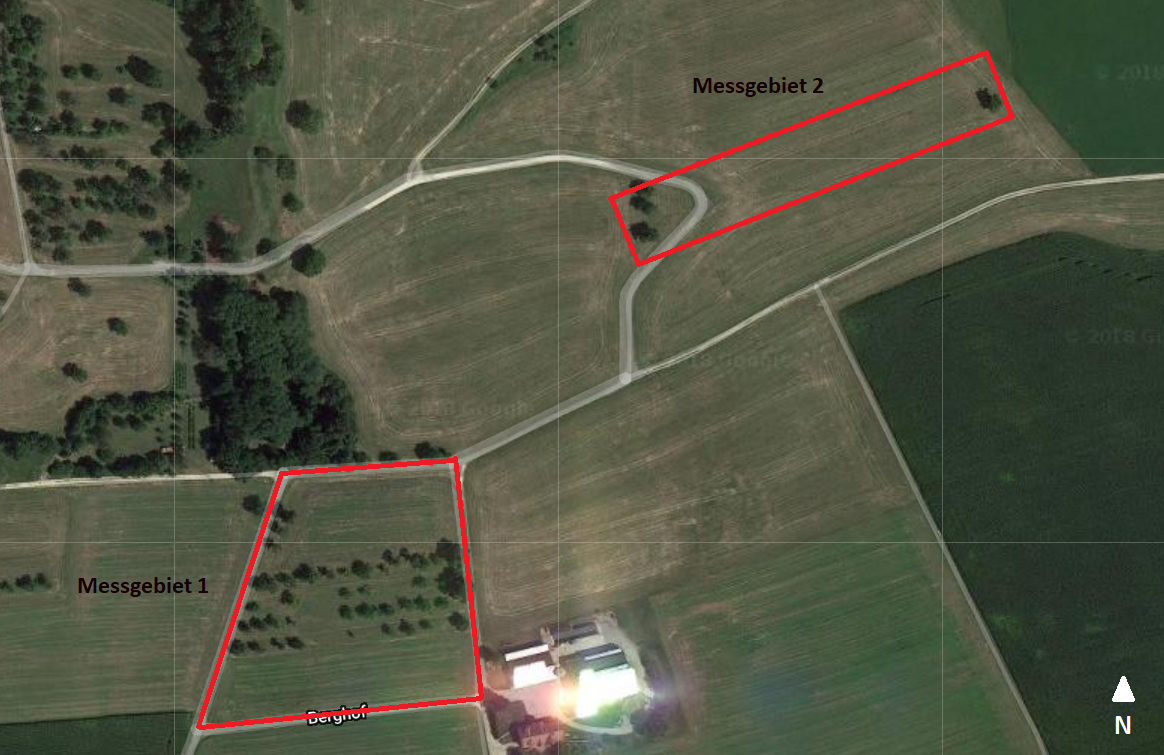
\includegraphics[width=0.9\textwidth]{fig/Messgebiete.png}
 \caption[Messgebiete]{Messgebiete auf denen unsere Messungen durchgeführt wurden. Unter Messgebiet 1 ist der Basaltgang. Die Graphik wurde von Rebekka Kirchgässner und Luisa Rank übernommen.}
 \label{abb:Messgebiete}
\end{figure}

Aberhalb den Messgebiets 1 ist eine Steinbruch in dem Basalt frei gelegt ist. Der Aufschluss dieses Basaltgangs ist etwa 5 Meter hoch und 16 Meter breit. 
Es ist zu erkennen, dass der Basalt nicht im ganzen Aufschuss in gleichem Zustand vorliegt. In der Mitte sieht er wesentlich kompakter aus als an den Rändern.
Dieser Basaltgang geht unterirdisch weiter und läuft schräg durch das Messgebiet 1. Bei den meisten unserer Messungen wurde der Basaltgang untersucht.

\begin{figure}[h]
 \centering
 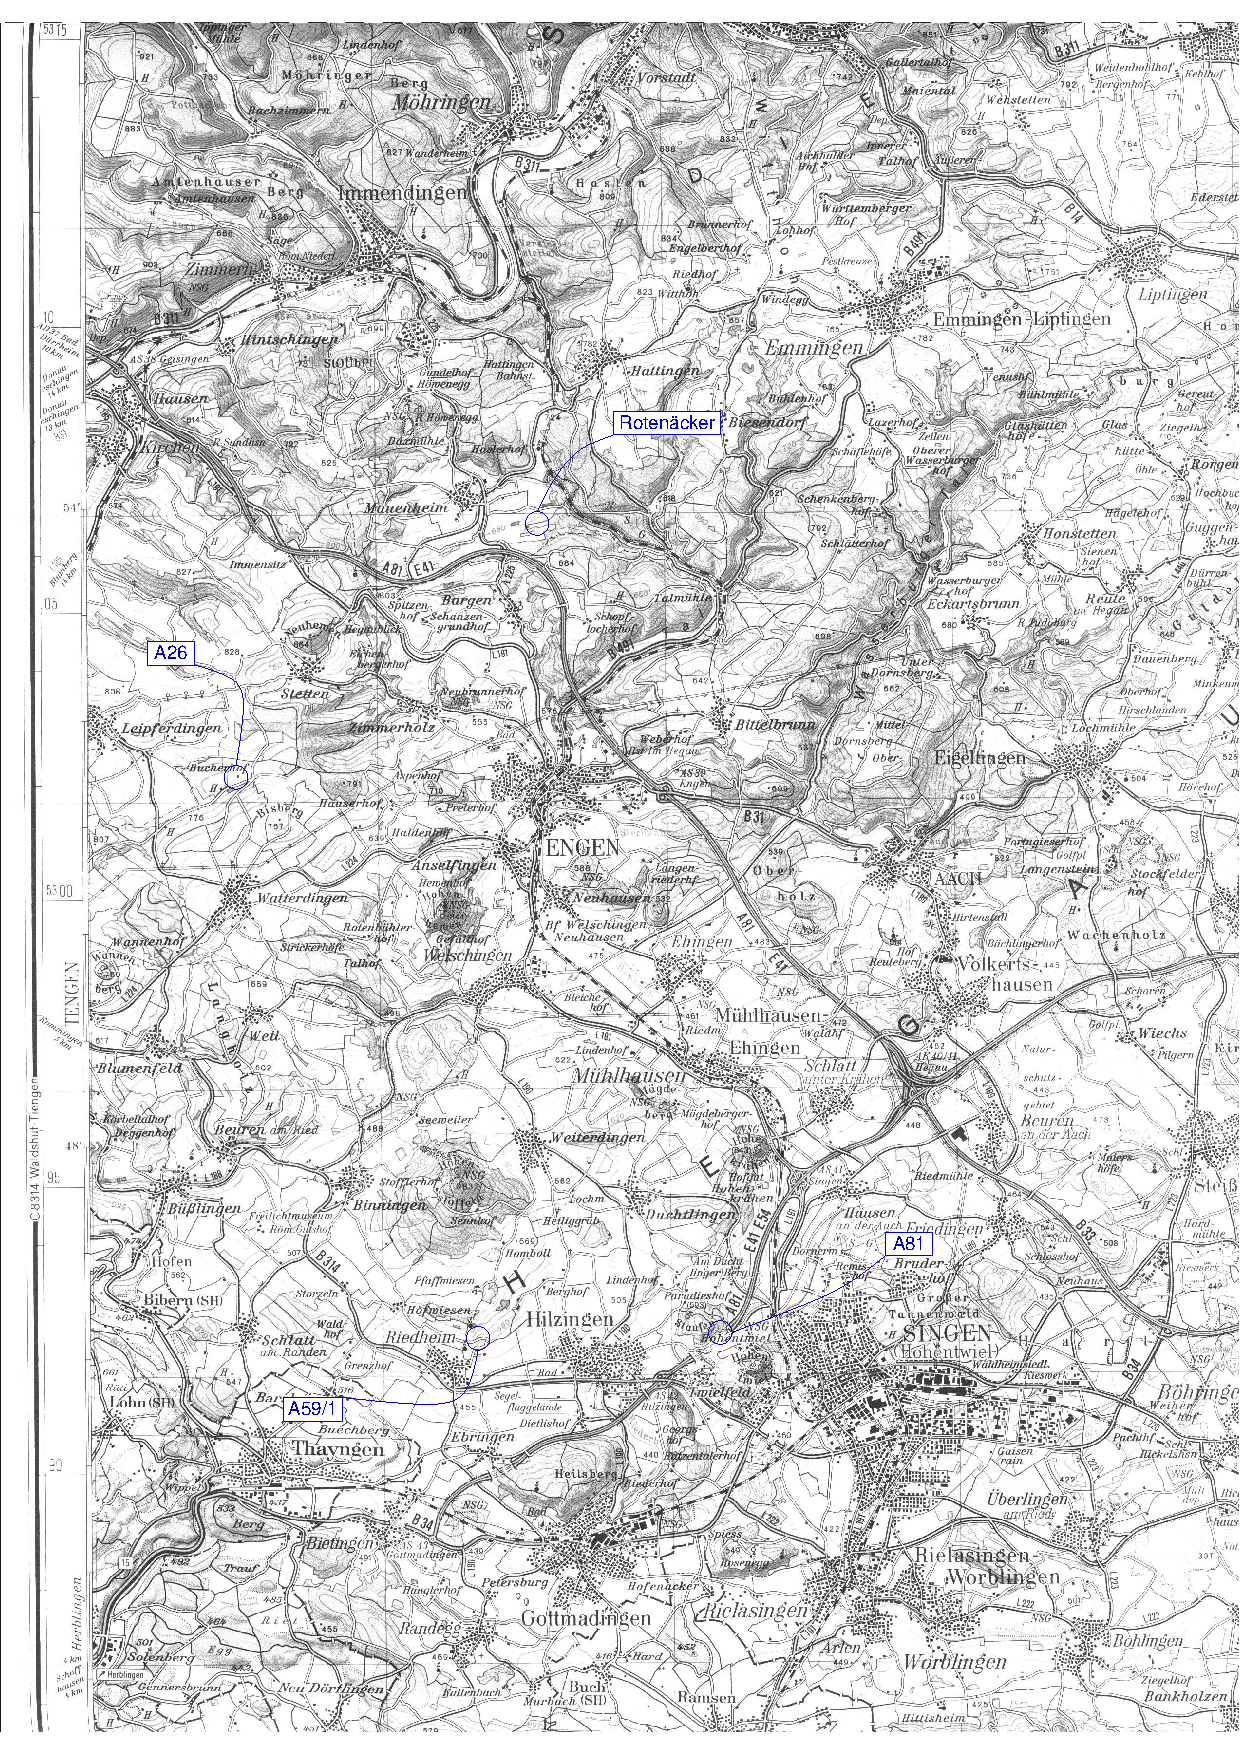
\includegraphics[width=0.9\textwidth]{fig/Uebersichtskarte der Messgebiete.pdf}
 \caption[Messgebiete]{Messstandorte auf denen die Geländeübung durchgeführt wurde. Unser Messstandort Riedheim ist unten links (A59/1) eingezeichnet.}
 \label{abb:Messgebiete}
\end{figure}

In Abbildung \ref{abb:Geolog} ist eine Geologische Karte unseres Messgebiets zu sehen. In der Mitte ist in schwarz der Basaltgang oberhalb des Steinbruchs zu sehen, denn dort wurde er sicher nachgewiesen.
Unterhalb des Steinbruchs ist die Lage des Basaltgangs durch zwei gestrichelte Linien angegeben, da hier nicht eindeutig nachgewiesen wurde ob es sich um Basalt handelt. Der Untergrund unter dem Messgebiet 1 besteht nach dieser Karte aus älterem Juranagelfluh. Dies wurde der Legende der Karte entnommen. Das Messgebiet 2 liegt teilweise über älterem Juranagelfluh und oberer Süßwassermolasse.

\begin{figure}
 \centering
 \includegraphics[width=0.9\textwidth]{fig/Geolog.pdf}
 \caption[Geologische Karte]{Geologische Karte des Messstandorts Riedheim}
 \label{abb:Geolog}
\end{figure}


